\chapter{基于单张自然环境照片的人脸重建}
\label{chap:recon}

\section{总体目标}

\section{基于神经网络回归的模型初始化}

\section{模型裁剪边缘的梯度处理}
可微分渲染在应用到人脸3D重建时有一个特殊的问题:人是一个很大的物体,而人脸重建的目标通常仅仅是人脸的这一小块区域。
所以通常在人脸重建中用于逆渲染的模型都是裁剪过的,只包含人脸的部分,因此具有一些人为制造的边缘。
这些边缘在照片中并不存在,但第\ref{chap:method}章提出的方法在应用到人脸时却也会在这些边缘产生相关梯度,由于并无对应的边缘可供对齐,这些梯度将导致模型过度扩展,影响最终收敛的效果。

解决该问题的关键在于如何判断渲染图像中的像素与模型指定边缘的位置关系,以便在计算梯度时能够区分人为制造的边缘和真正需要优化的边缘。
对此,本文受到\citet{sdf_glyphs}的启发,该作者提出使用SDF(Signed Distance Field,有向距离场)贴图来绘制可任意放大的矢量图形,并能根据SDF的梯度判断像素到图形边缘的距离,从而实现各向异性的抗锯齿。
于是,本文提出一种简单的基于SDF贴图的方法来区分人为制造的和真正需要优化的边缘。

具体地,本文定义一种SDF贴图。
对于该贴图中的每个像素,其值为一个单通道浮点数$d$,表示该像素点到最近的人为制造边缘的距离,在模型内部的为正,模型外部的为负,
如图\ref{fig:sdf}所示。
由于该贴图中并无太多高频信息,本文仅使用了$256 \times 256$的分辨率。
虽然似乎只有模型内部的贴图像素才会在渲染时被采样到,只需要计算模型内部的正值即可,但实际上,由于采样时使用双线性插值,外部的负值也会被采样到从而参与插值计算中.
更准确的线性插值结果正是SDF的主要优势之一。
从图中也可见,无论是SDF值还是其梯度在穿过边缘时都依然是平滑的。

\begin{figure}
\centering
\begin{subfigure}[t]{3.3in}
    \centering
    \import{build/figures}{sdf.pgf}
    \caption{SDF贴图}
    \label{fig:sdf}
\end{subfigure}
\begin{subfigure}[t]{2.9in}
    \centering
    \import{build/figures}{sdf_grad.pgf}
    \caption{SDF的梯度}
    \label{fig:sdf_grad}
\end{subfigure}
\caption[SDF贴图可视化]{SDF贴图可视化。灰色线为模型中人为制造的边缘。(a)为SDF贴图,表示每个像素到最近边缘的距离,模型内部为正,外部为负;(b)为(a)的梯度向量,其x和y分量分别可视化为红色和绿色通道。}
\end{figure}

下面以nvdiffrast的工作方式为例说明该贴图的使用方式:
nvdiffrast抗锯齿模块工作时将以一对相邻的像素点为单位(如图\ref{fig:aa}),其中一个像素在模型内部,另一个像素在模型外部。
对于处于模型内部的像素,可从SDF贴图中采样其对应的$d$值,并计算$\frac{\partial d}{\partial \mathbf{x}}$,其中$\mathbf{x}$为对应外部像素相对该内部像素的坐标偏移量。
也即对3D模型的表面在该内部像素点的位置使用一个平面进行一阶近似,并求外部像素在该近似平面上的位置,以估计外部像素是否在人为制造边缘之外。
正式地,对于一对分别处于模型内外的像素点,其处于人为制造的边缘当且仅当:
\begin{equation}
    d + \max\left(a\frac{\partial d}{\partial \mathbf{x}}, \delta\right) < 0
    \text{,}
\end{equation}
此时应该忽略其产生的可见性梯度。其中$\delta=0.1$为人为限制的梯度的最大值,为避免小概率时过大梯度产生过于离谱的结果;$a=1.5$为梯度放大的系数,为避免偶发的由于精度不足导致的检测遗漏。
这两个超参数的选择对最终结果的影响不大。

\begin{figure}
\centering
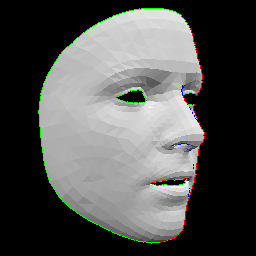
\includegraphics[height=2.2in]{figures/debug_sdf}
\caption[人为制造边缘分类效果]{人为制造边缘分类效果。绿色为人为制造的边缘;红色为与未知背景间的边缘;蓝色为模型内部相互遮挡产生的边缘。}
\label{fig:sdf_result}
\end{figure}

该算法对边缘分类的效果如图\ref{fig:sdf_result}所示。
可见算法将所有边缘分为了三类,
其中绿色为人为制造而需要忽略的边缘,
红色为与未知背景间的边缘,可按照第\ref{chap:method}章提出的方法进行处理,
蓝色为模型内部相互遮挡产生的边缘,应按正常可微分渲染流程处理。
从图中可见一些红色与绿色交错的区域,这是由于这两种边缘本身并没有明确的界限,有时人为制造的边界会正好投影到实际边界附近。
因此本文认为这种现象是十分合理且可接受的。

\paragraph{SDF贴图的计算}
关于SDF的计算方法有很多,下面介绍本文的实现方式。
本文首先使用Blender将3D人脸模型展开至纹理空间,然后在展开后的所有三角形中查找仅属于一个三角形的边做为所谓人为制造的边缘。
并将这些边加入CGAL封装的层次包围盒\footnote{https://doc.cgal.org/latest/AABB\_tree/index.html}数据结构中,以便快速查找。
随后调用OpenGL将所有展开后的三角形光栅化渲染至图像中,得到边缘内部像素的遮罩。
最后,对于贴图中的每个像素,从层次包围盒中查找与其最近的边,计算其与该边的距离$|d|$,并根据遮罩赋予其符号。$d$的梯度方向即为从该像素指向该边上与其最近点的方向(或反方向),模长为$1$。
本方法相比\citet{sdf_glyphs}介绍的暴力方法效率更高,本方法计算$256\times256$分辨率的贴图,使用CPU单线程用时在10毫秒左右。

\paragraph{梯度计算}
梯度$\frac{\partial d}{\partial \mathbf{x}}$的计算与所使用的渲染方式有关。
例如OpenGL支持通过数值方法直接求任意变量关于像素坐标的梯度\footnote{https://registry.khronos.org/OpenGL-Refpages/gl4/html/dFdx.xhtml}。
而针对本文使用的nvdiffrast来说,本文首先以解析法随SDF一同计算其关于纹理坐标的梯度$\frac{\partial d}{\partial u}$和$\frac{\partial d}{\partial v}$,并将其与$d$一同保存于贴图中。
然后根据nvdiffrast的插值模块给出的纹理坐标和像素坐标间的雅可比矩阵将其到像素坐标:
\begin{equation}
    \begin{bmatrix}
        \frac{\partial d}{\partial x} \\
        \frac{\partial d}{\partial y}
    \end{bmatrix} = \begin{bmatrix}
        \frac{\partial u}{\partial x} & \frac{\partial u}{\partial y} \\
        \frac{\partial v}{\partial x} & \frac{\partial v}{\partial y}
    \end{bmatrix} \begin{bmatrix}
        \frac{\partial d}{\partial u} \\
        \frac{\partial d}{\partial v}
    \end{bmatrix}
\text{。}
\end{equation}
该方法与\citet{sdf_glyphs}中提出的方法相同。
所要求的$\frac{\partial d}{\partial \mathbf{x}}$根据前景和背景像素的相对位置,是$\frac{\partial d}{\partial x}$或$\frac{\partial d}{\partial y}$或其相反数四者之一。

另一种解决该问题的可能的方案是屏蔽位于模型表面特定区域的像素上的可见性梯度,例如屏蔽特定三角形,屏蔽到边缘距离小于某个阈值的区域,手动指定遮罩等。
相比于这些方法,本方法具有如下优势:
\begin{enumerate}
\item 渲染尺度无关:同样的模型区域在不同尺度下渲染呈现的尺度不同,因此屏蔽区域的选择可能需要随着尺度变化而改变。
而本方法融入$d$了对像素坐标的梯度信息,是模型表面的一阶近似,因此不受尺度的影响。
\item 有向性:即使是同一个像素,在其不同方向上也可能分别靠近不同种类的边缘。
本方法通过考虑$d$的梯度方向,可以区分这些不同的边缘。
\end{enumerate}

\section{照片到纹理空间信息迁移}

\section{基于可微分渲染的3D重建}

\section{实验结果}

\section{局限性}
